

\chapter{\selfour Basics}
\label{chap:sel4}

So far we have provided a general background on real-time scheduling and resource sharing.
As the final piece of background we now present an overview of the concepts relevant to the temporal behaviour of our implementation platform, \selfour.

\selfour is a microkernel that is particularly suited to safety-critical, real-time systems
with one major caveat: time is not treated as a first-class resource, and as a result support for
temporal isolation is deficient. Three main features of \selfour
support this claim: it has been formally verified for correctness~\citep{Klein_EHACDEEKNSTW_09,
Klein_AEMSKH_14}, integrity~\citep{Sewell_WGMAK_11}, confidentiality~\citep{Murray_MBGBSLGK_13}.
; All memory management, including kernel memory, is at
user-level~\citep{Elkaduwe_Derrin_06}; Finally it is the only \gls{OS} to date with full \gls{WCET}
analysis~\citep{Sewell_KH_16}.  

In this section we will present the current state of relevant \selfour features in order to
highlight deficiencies and motivate our changes.  We present the capability system, resource
management, communication including \gls{IPC} and the scheduler, followed by an analysis of
how the current mechanisms can be used in real-time systems.

First we introduce the powerful \selfour capability system, used to access all resources in the
system---with the exception of \emph{time}. The scheduler in \selfour has been left intentionally
underspecified~\citep{Petters_EH_12} for later work.  The current implementation is a place holder,
and follows the traditional L4 scheduling model~\citep{Ruocco_06}---a fixed-priority, round-robin
scheduler with 256 priorities. 


\section{Capabilities}
\label{s:capabilities}

As a capability-based \gls{OS}, access to any resource in \selfour is via capabilities (recall
\Cref{s:os-capabilities}). Capabilities to all system resources are available to the initial task---the first
user-level thread started in the system---which can then allocate resources as appropriate.
Capabilities exist in a \emph{capability space} that can be configured per thread or shared between
threads. 

Capability spaces (\code{cspace}s) are analogous to address spaces for virtual memory: where address spaces map
virtual addresses to physical addresses, capability spaces map object identifiers to access rights.
Cspaces are formed of \emph{capability nodes} \code{cnode}s which contain capabilities, analogous to page tables
in virtual memory, and can contain capabilities to further \code{cnode}s, which allows for multi-level
cspace structure. A cspace address refers
to an individual entry in some CNode in the capability space, and may be empty or contain a
capability to a specific kernel resource. For brevity, a cspace address is referred to as
a \emph{slot}. 

% access rights
Each capability has three potential access rights: read, right and grant. How those rights affect
the resource the capability provides access to depends on the type of resource, and is explained in
the next section.

\begin{table}
    \centering
    \rowcolors{2}{gray!25}{}
    \begin{tabularx}{\textwidth}{lX}\toprule
    \emph{Operation}    & \emph{Description}\\\midrule
    \code{Copy}         & Create a new capability in a specified CNode slot, which is an exact copy
                         of the other capability and refers to the same resource. \\
    \code{Mint}         & Like copy, except the new capability may have diminished rights and/or be
                          badged. \\
    \code{Move}         & Move a capability from one slot to another slot, leaving the previous slot
                          empty. \\
    \code{Mutate}       & Like move, except the new capability may have diminished rights and/or be
                          badged. \\
    \code{Rotate}        & Atomically move two capabilities between three specified slots. \\
    \code{Delete}        & Remove a capability from a slot. \\
    \code{Revoke}        & Delete any capabilities derived from this capability. \\
    \code{SaveCaller}    & Saves the kernel generated resume capability into the designated slot. \\
    \bottomrule 
    \end{tabularx}
    \caption{Summary of operations on capabilities provided by baseline \selfour~\citep{seL417}}.
    \label{t:capability_ops}
\end{table}

% badges and operations
Various operations can be done on capabilities, which are summarised in \cref{t:capability_ops}.
When a capability is copied or minted, it is said to be \emph{derived} from the original capability.
All derived capabilities can be deleted by using \code{revoke}.
There are restrictions on which capabilities can be derived and under what conditions, depending on
what the capability provides access to. 
\emph{Badging} is a special type of derivation which allows specific capability types to be copied
with an unforgeable identifier. We discuss derivation restrictions and the use of badges further
in this chapter.
Any individual capability can be deleted, or revoked. The former simply removes a specific
capability from a capability space, the latter removes all child capabilities.

\section{System calls and invocations}

\selfour has a two-level system call structure, based on capabilities. The first level of system
calls, listed in \cref{t:system-calls}, are distinguishable by system call number.  The majority of
system calls are for communication; \code{send}, \code{nbsend}, \code{call}, \code{reply} are for
sending messages; \code{recv}, \code{nbrecv} for receiving messages; and \code{yield} for
interacting with the scheduler. An \code{nb} prefix indicates that this system call will not block.

Second-level system calls are called \emph{invocations} and are modelled as sending a message
to the kernel. All invocations are conducted by a sending system call. The kernel is modelled as if
it is waiting for a message and receives one every time a system call is made, and sends a message
as a reply. 
To determine the operation, the rest of the arguments to an invocation are encoded as a message to
the kernel. Each capability type has a different set of invocations available, and on kernel entry 
 the invoked capability is decoded to determine the action the kernel should take. 

\begin{table}[t] 
    \centering
    \begin{tabularx}{\textwidth}{llXl}\toprule
        \emph{System call}                          & \emph{Parameter}     & \emph{Description}
        & \emph{Return?} \\\midrule
        \rowcolor{gray!25} \texttt{send, nbsend}    & \texttt{dest} & Capability to invoke. & \no     \\
        \rowcolor{gray!25}                          & \texttt{info} & Description of message. & \\     
        \texttt{call}              & \texttt{dest}  & Capability to invoke. & \\
                                   & \texttt{info}  & Description of message.   & \yes \\
        \rowcolor{gray!25}
        \texttt{recv, nbrecv}      & \texttt{src}   & Capability to block on. & \yes \\
        \rowcolor{gray!25}
                                   & \texttt{badge} & Destination for badge. & \\
        \texttt{reply}             & \texttt{info}  & Description of reply message. & \no\\
        \rowcolor{gray!25}
        \texttt{replyrecv}         & \texttt{info}  & Description of reply message. &\yes\\
        \rowcolor{gray!25}
                                   & \texttt{src}   & Capability to block on. &        \\
        \rowcolor{gray!25}
                                   & \texttt{info}  & Description of reply message. & \\
        \rowcolor{gray!25}         & \texttt{badge} & Destination for badge. &        \\
        \texttt{yield}             & \no            & \no                             \\
        \bottomrule
    \end{tabularx}
    \caption{\selfour system call summary. All system calls except \code{yield} are based on sending
    and/or receiving messages. The \emph{return} column indicates if a system call returns a message
or not.}
    \label{t:system-calls}
\end{table}

All the operations on capabilities are that are listed in \cref{t:capability_ops} are invocations
on \code{cnode} capability addresses. For example, to copy a capability, one uses \code{call} on a
\code{cnode}, and provides the invocation code for copy, as well as the arguments. In the case of
copy, one provides the slot of the capability being copied, in addition to the destination
\code{cnode} and
slot. 

\section{Physical memory management}

All kernel memory in \selfour is managed at user-level and accessed via capabilities,
which is key to \selfour's isolation and security, but also essential for
understanding the complexity of kernel design. Additionally, this allows for the ultimate in policy
freedom: all resource allocation is done from user-level by those holding the appropriate
capabilities. Capabilities to kernel memory contain a physical address and a type which indicates
what type of memory is at that physical address. Options for different types are shown in
\cref{t:kernel_objects}. 

% table of object types 
\begin{table}[t]
    \centering
    \rowcolors{2}{gray!25}{}
    \begin{tabularx}{\textwidth}{p{3cm} X}\toprule
    \emph{Object}    & \emph{Description}\\\midrule
    Untyped          & Memory that can be retyped into other types of memory, including untyped.\\
    CNode            & A fixed size table of capabilities. \\
    \Gls{TCB}        & A thread of execution in \selfour.\\
    Endpoint         & Ports which facilitate \gls{IPC}. \\
    Notification object & Arrays of binary semaphores.\\
    Page Directory  & Top level paging structure. \\
    Page Table      & Intermediate paging structures.\\
    Frame           & Mappable physical memory. \\
    \bottomrule
    \end{tabularx}
    \caption{Major memory object types in \selfour, excluding platform specific objects. For further detail
    consult the \selfour manual~\citep{seL417}}.
     \label{t:kernel_objects}
\end{table}

In the initial system state, capabilities to all resources are given to the first task started by
the system, the \emph{root task}. Then according to system policy the root task can divide up and
delegate system resources.  This includes capabilities to all memory, apart from the small section
of static memory used by the kernel. The kernel itself has a large, static \emph{kernel window}
initialised at boot time, which
consists of memory mapped such that it is directly writeable by the kernel. The kernel window size
is platform specific, but is 500MiB on all 32-bit platforms.  

\subsection{Untyped}

All memory starts as \emph{untyped} memory, and capabilities to all available untyped memory are placed in the
cspace of the root task on boot. Each untyped consists of a start address, a size, and a flag
indicating whether the untyped is writeable by the kernel or not. Memory reserved for devices and
memory outside the kernel window is not readable or writeable by the kernel: the rest is untyped
memory, free for use by the system. 

Untyped objects have only one invocation: \emph{retype}, which allows for large untyped objects to
split into smaller objects of a different size and type, including frames, page tables, cnodes, etc. 
While the majority of objects in \selfour have a platform-dependent size fixed at compile time, some
are sized dynamically at runtime, \eg untyped and CNodes, which can be any power of two size.

Any capability to memory---untyped or not---is a capability to a specific object in memory,
containing a pointer to that object. When retype is used to create sub-objects in from an untyped
object, those
subsets of memory will not become available for retyping again until every capability to that object has been deleted, somewhat like reference counting pointers.

\Cref{t:untyped} shows an example initial memory layout for the \textsc{Sabre} platform, which has a
500MiB kernel window. Physical memory on this platform starts at 0x10000000, which is mapped into
the kernel address space at 0xe0000000. Physical addresses outside of this range are devices and
are not writeable by the kernel.
Capabilities to all available memory and devices are set up as untyped in the initial root task's
\code{cnode}. 

\begin{table}[b] 
    \centering
    \rowcolors{2}{gray!25}{}
    \begin{tabularx}{\textwidth}{llX} \toprule
        \emph{Start physical address} & \emph{End physical address} & \emph{Kernel virtual address} \\\midrule
    0x100000   & 0x2c00000   & \no \\
    0x10000000 & 0x10010000 & 0xe0000000 \\
    0x105c3000 & 0x2f000000 & 0xe105c3000 \\
    0x2f106400 & 0x2fdfc200 & 0xff106400 \\
    \bottomrule
    \end{tabularx}
    \caption{Initial memory ranges on at boot time on the \textsc{Sabre} platform.}
    \label{t:untyped}
\end{table}


\subsection{Virtual Memory}

Page tables, intermediate paging structures and physical frames are all created by retyping
untyped objects. Page tables and frames have a set of architectural invocations including mapping, 
unmapping, and cache flushing operations.

\subsection{Thread control blocks}

\Glspl{TCB} represent an execution context and manage processor time in \selfour, and consist of a
base TCB structure and a \code{cnode}. 
The base TCB structure contains accounting information for scheduling and IPC in addition to the
register set and floating-point context. 
The \code{cnode} contains capabilities that should not be
deleted while a thread is running
leveraging the fact that an object cannot be truly deleted until all capabilities to it are removed.
These capabilities include the top-level \code{cnode}, top-level page directory, and three
capabilities for \gls{IPC}. 
\cref{t:tcb_ops} shows the main invocations possible on TCB capabilities.

% table of tcb invocations
\begin{table}[b]
    \centering
    \rowcolors{2}{gray!25}{}
    \begin{tabularx}{\textwidth}{lX}\toprule
    \emph{Operation}    & \emph{Description}\\\midrule
        \code{Resume}               & Place a thread in the scheduler.\\ 
        \code{Suspend}              & Remove a thread from the scheduler.\\
        \code{WriteRegisters}       & Configure a thread's execution context.\\
        \code{ReadRegisters}        & Read a thread's execution context.\\
        \code{SetAffinity}          & Set the CPU on which this thread should run.\\
        \code{SetIPCBuffer}         & Set the page to use for the IPC buffer.\\
        \code{SetPriority}          & Set the priority of this TCB.\\
        \code{BindNotification}     & Bind this TCB with a notification object (see
        \cref{s:notification-binding}). \\
    \bottomrule 
    \end{tabularx}
    \caption{Summary of operations on \glspl{TCB}. Further operations are available that batch several
    setters to reduce thread configuration overheads.}.
     \label{t:tcb_ops}
\end{table}

\subsection{Endpoints}
\label{s:endpoints}

Endpoints are the general communication port used by \selfour for \gls{IPC}.
Any thread with a
capability to an endpoint can send and receive messages on that endpoint, subject to the access
rights. Endpoints are small, and consist of the endpoint badge, some state information and a queue
of threads blocked on the endpoint. We cover how endpoints interact with IPC in the upcoming
\cref{p:sel4_ipc}. 

\subsection{Notifications}

Notification objects are an array of binary semaphores used to facilitate asynchronous communication in \selfour, either from other threads via \texttt{send()} or from
interrupts. Notification objects consist of a queue of blocked threads and a word of information,
which contains the semaphore state. Further information on notifications is presented in
\cref{p:sel4_notifications}. 

\subsection{Consequences}

User-level management of kernel memory provides true policy freedom---there is no
policy required by the kernel on memory layout---this design is not without trade-offs. Ultimately,
user-level management of kernel memory is key to \selfour's isolation
guarantees as system designers can fully partition systems by using specific memory layouts and
avoid shared structures determined by the kernel itself. However, there are two major impacts on kernel 
design: back-pointers, and dynamic data structures. 

The fact that any capability may be deleted at any time means that any pointer between two memory
objects must be doubled, with pointers from each object to each other, as any object must be able to be
traversed on order to reach any other linked object. This is analogous to a doubly-linked list,
where for $O(1)$ deletion from any node in the list, the list must have pointers in both directions.
This increases performance of deletion but also doubles the memory required for each list node. 

Secondly, because of the policy freedom, the kernel has no limits on resources, meaning no memory
resource can be statically sized. Consequently, simple, static data structures, like arrays, cannot
be used in the kernel as no assumptions on memory layout can be made, meaning dynamic data
structures are mandated. Because the kernel cannot make assumptions about the location of memory
objects, specific optimisations are also not possible: it is up to the system designer to decide a trade-off
between isolation and efficiency in the memory layout of the system.

Both of these consequences make for restrictions on kernel design, which can be demonstrated through
the list of TCBs maintained by the kernel scheduler. Each priority in the scheduler has a
doubly-linked list of TCBs: although the scheduler itself only ever removes the head of the list,
which is $O(1)$ on a singly-linked list, a doubly-linked list is required as TCB objects can be
deleted at any time. Memory placement of TCBs impacts scheduler performance, as depending on
allocation patterns, different list nodes may trigger cache misses or worse, cache conflicts. As a
result, the scheduler will perform far worse than a static, array-based scheduler using a fixed
maximum number of TCBs with known ids for indexing. However, such an approach provides no policy
freedom, and is more suitable at a middle-ware level in the \gls{OS} implemented on top of the
microkernel. 

\section{Control capabilities}
\label{s:control-capabilities}

Not all capabilities refer to memory-based resources, such as interrupts and \IO ports.
In order to obtain capabilities to specific interrupts or ranges of \IO ports, the root task is
provided with non-derivable control capabilities which can be invoked to place specific hardware
resource capabilities in empty slots.

\begin{table}
	\centering
    \rowcolors{2}{gray!25}{}
    \begin{tabularx}{\textwidth}{lX|lX} 
        \toprule
        \emph{Slot(s)}  & \emph{Contents} & \emph{Slot(s)} & \emph{Contents} \\\midrule
        0          & empty &
        8          & \code{IO\_space\_control} \\
        1          & initial thread's TCB &
        9          & initial thread start-up information frame \\
        2          & this \code{cnode} &
        10         & initial thread's IPC buffer frame \\
        3          & initial thread's page directory &
        11         & \code{domain\_control} \\
        4          & \code{irq\_control} &
        12---18    & initial thread's paging structures \\
        5          & \code{ASID\_control} &
        19---1431  & initial thread's frames \\
        6          & initial thread's ASID pool &
        1431---1591 & untyped \\
        7           & \code{IO\_port\_control} &
        1592---($2^{16}-1$) & empty \\
        \bottomrule
	\end{tabularx}
    \caption{Slot layout in the initial \code{cnode} set up by the kernel for the root task on the
\textsc{Sabre}.}
	\label{t:initial_cnode}
\end{table}

\cref{t:initial_cnode} shows the root tasks initial cspace layout as set up by the kernel for the
\textsc{Sabre} platform. Apart from capabilities to memory objects for the root task and the
remaining untyped, the initial \code{cnode} contains five control capabilities for managing
interrupts, \glspl{ASID}, \IO Ports, \IO Spaces and domains.

We take interrupts as an example to explain how control capabilities function. The
\code{irq\_control} capability is the control capability for obtaining capabilities to specific
interrupt numbers. By invoking the \code{irq\_control} capability, users can obtain IRQHandler
capabilities to specific interrupt numbers, thereby granting them authority to invoke that handler.
Once an IRQHandler capability is obtained, users can invoke it to manage that specific interrupt.
On x86, \code{irq\_control} is also used to provide capabilities to model specific registers and \IO
interrupts.

\section{Communication}

\selfour provides communication through synchronous IPC via endpoints, or asynchronous notifications
via notification objects. All the communication system calls introduced in \cref{t:system-calls},
when used on endpoints and notifications, are used to communicate between TCBs. There are no
invocations that can take place via endpoints or notification capabilities. 

\subsection{IPC}
\label{p:sel4_ipc}

IPC in \selfour consists of threads sending and receiving messages in a blocking or non-blocking
fashion over endpoints, which act as
message ports. Each thread has a buffer (referred to as the \emph{IPC buffer}), which contains the payload of the message, consisting
of data and capabilities. Senders specify a message length and the kernel copies this (bounded)
amount between the sender and receiver IPC buffer. Small messages are sent in registers and do not
require a copy operation. 
Along with the message the kernel additionally delivers the badge of the endpoint capability that the sender 
invoked to send the message.

\begin{figure}[t]
    \centering
    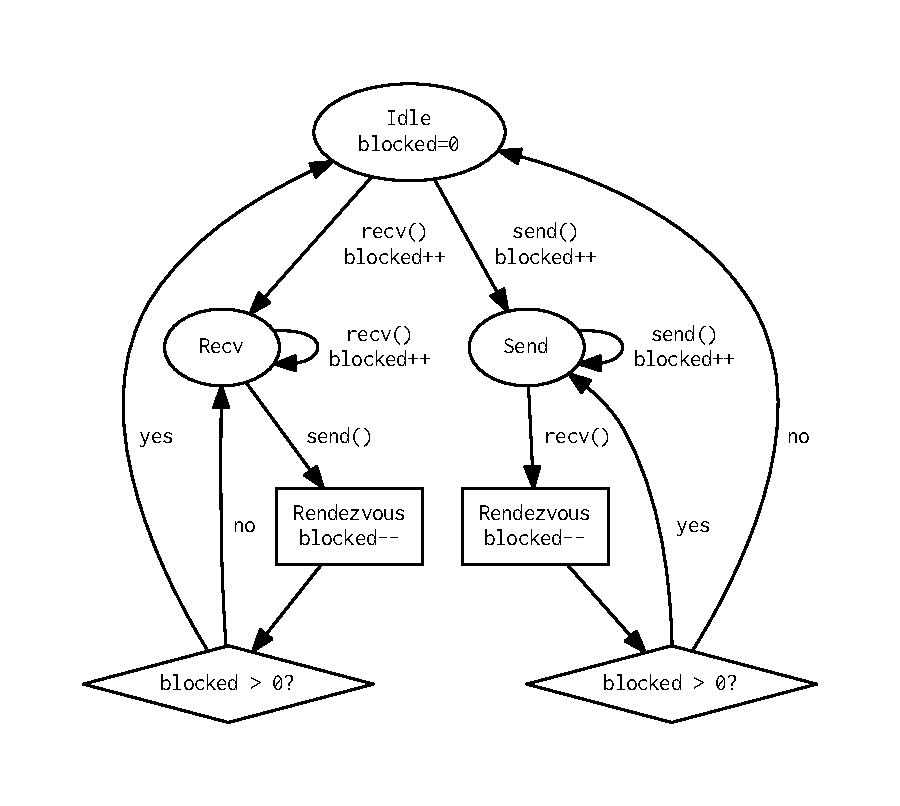
\includegraphics[width=0.8\textwidth]{endpoint}
    \caption{State diagram of a single endpoint, where \emph{blocked} tracks the number of threads
    waiting to send or receive. Note that only one list of threads is maintained by the endpoint:
senders and receivers cannot be queued at the same time.}
    \label{f:endpoint}
\end{figure}


IPC can be one-way, where a single message is sent between a sender and receiver, or two-way in an
RPC fashion where the sender sends a message and expects a reply. \emph{IPC rendezvous} refers to
when the IPC takes place, specifically when the kernel transfers data and capabilities between two
threads. 

\begin{table}[t]
    \centering
    \rowcolors{2}{gray!25}{}
    \begin{tabularx}{\textwidth}{lX}\toprule
        \emph{System call} & \emph{Action} \\\midrule
        \texttt{send}   & Send a message, blocking until it is consumed. \\ 
        \texttt{nbsend} & Send a message, but only if it is consumed immediately (\ie a thread is
        already waiting on this endpoint for a message).  \\
        \texttt{recv}   & Block until a message is available to be consumed from this endpoint.  \\
        \texttt{nbrecv} & Poll for a message---consume a message from this endpoint, but only if it is available
        immediately.   \\
        \texttt{call}   & Send a message, and block until a reply message is received. \\
        \texttt{reply}  & Send a reply message to a \code{call}.   \\
        \texttt{replyrecv} & Send a reply message to a \code{call} and then \code{recv}. \\
        \bottomrule
    \end{tabularx}
    \caption{System calls and their effects when used on endpoint capabilities.}
    \label{t:endpoint-system-calls}
\end{table}

Table \cref{t:endpoint-system-calls} summarises \selfour system calls when used on endpoint
capabilities. Essentially, \code{send()} is used to send a message and \code{recv()} used to
receive one, both having blocking and non-blocking variants. \code{call()} is of particular interest as it represents the caller side of an RPC
operation critical to microkernel performance, distinguished from a basic pair of \code{send()} and
\code{recv()} by \emph{resume} capabilities. Pioneered in EROS~\citep{Shapiro_SF_99}, resume
capabilities are generated once the message sent by \code{call()} is consumed, and consist of the
thread waiting for a reply message. In \selfour, the resume capability is stored in the \gls{TCB}
\code{cnode}, and \code{reply()} is the operation used to invoke this capability and send the reply
message back.

\begin{figure}
    \centering
    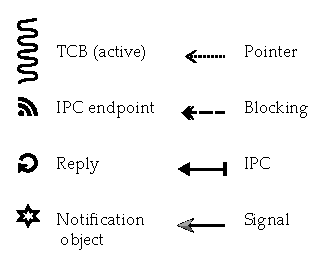
\includegraphics[width=0.5\textwidth]{legend-1}
    \caption{Legend for diagrams in this section}
    \label{f:legend-1}
\end{figure}


\begin{figure}
    \centering
    \begin{subfigure}[h]{0.48\textwidth}
        \centering
        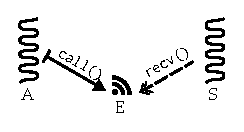
\includegraphics[width=\textwidth]{ipc1}
        \caption{Initial IPC rendezvous}
        \label{f:ipc1}
    \end{subfigure}%
    \begin{subfigure}[h]{0.48\textwidth}
        \centering
        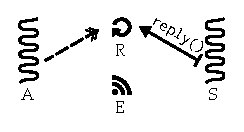
\includegraphics[width=\textwidth]{ipc2}
        \caption{Reply phase}
        \label{f:ipc2}
    \end{subfigure}
    \caption{IPC phases: a TCB, $A$ sends a message to endpoint $E$ using \code{call()}. Another
        TCB, $S$, blocks on $E$ using \code{recv()}. At this point the message is transferred from 
        $A$ to $S$ and $A$ is blocked the reply capability. (b) shows the
    reply phase, where $S$ uses \code{reply()} to send a reply message to $A$, waking $A$. See \Cref{f:legend-1} for the legend.}
    \label{f:ipc}
\end{figure}

% notifications, interrupts, aep-binding
\begin{figure}
    \centering
    \begin{subfigure}[h]{0.48\textwidth}
        \centering
        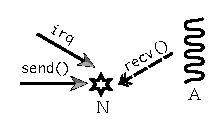
\includegraphics[width=\textwidth]{signal1}
        \caption{Notifications.} 
        \label{f:signal1}
    \end{subfigure}%
    \begin{subfigure}[h]{0.48\textwidth}
        \centering
        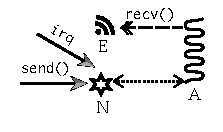
\includegraphics[width=\textwidth]{signal2}
        \caption{Notification binding.}
        \label{f:signal2}
    \end{subfigure}
    \caption{Example of a thread, TCB $A$, receiving notifications, by blocking on the notification and by
        notification binding. In \cref{f:signal1} $A$ blocks waiting on notification
        object $N$, and wakes when any notifications or interrupts are sent to $N$. In
        \cref{f:signal2}, $A$ blocks on endpoint $E$, however since
        $N$ is bound to the $A$, if $N$ receives an interrupt or notification,
        $A$ is woken and the data word delivered to $A$.
        See \Cref{f:legend-1} for the legend.}
    \label{f:signal}
\end{figure}

\Cref{f:ipc1} demonstrates the rendezvous phase, where regardless of the order of operations, 
when one thread blocks (\code{recv()}) on the endpoint and another thread sends on that endpoint
then the message is consumed by the receiver. This occurs for both one-way and two-way \gls{IPC}.
Receivers can save
the \emph{resume} capability into their \code{cspace} to send a reply to later, but otherwise the resume capability is
installed in the \gls{TCB} CNode. The \emph{reply} system call directly invokes the resume
capability in this slot. 

Multiple senders and receivers can use the same endpoint, and which act as \gls{FIFO}
queues. In order to distinguish senders, receivers can use endpoint badges, which are unforgeable as
they are copied by the kernel directly. 

% fastpath
\subsection{Fastpath}

Recall from \cref{s:background-ipc} that \gls{IPC} performance is critical to a microkernel, which
is achieved through optimised fastpaths. A fastpath is an optimised code path for the most
performance critical operations. \selfour
contains two \gls{IPC} fastpaths which is used when the following, common-case conditions are satisfied:

\begin{enumerate}
    \item the sender is using \texttt{call()} or the receiver is using \texttt{replyrecv()},
    \item there are no threads of higher priority than the receiver in the scheduler,
    \item the receiver has a valid address space and has not faulted,
    \item and the message fits in registers.
\end{enumerate}

\subsection{Fault handling}

Fault handling in \selfour is modelled as IPC messages between the kernel and receivers. 
\glspl{TCB} can have a specific fault endpoint registered, on which the kernel can send simulated
\gls{IPC} messages containing information about the fault. Fault handling threads receive messages
on this endpoint as if the faulting thread had sent a message to that thread with \code{call()}. Of
course, this message is actually constructed by the kernel, and the message contains information
about the fault, generally the faulting thread's registers. The faulting thread is blocked on the
resume capability, which is generated, just as if the faulting thread had conducted a \code{call()}.
The fault handling thread can subsequently reply to this message to
resume the thread, although the reply message is also special: it can be used to reply with a new
set of registers for the faulting thread to be resumed with, and tell the kernel if it should
restart the thread or leave it suspended after the reply message is processed.
If no fault endpoint is present, the
thread is rendered inactive and no fault message is sent. 

\subsection{Notifications}
\label{p:sel4_notifications}

Notification objects provide the mechanism for semaphores in \selfour, and consist of a word of
data. Sending on a notification either sends the badge of the invoked notification capability to a 
thread waiting on that notification object, or if no threads are waiting stores, the badge in the
data word of the notifications. Unlike IPC, where messages being sent are queued, notifications
accumulate messages in the data word.

\begin{figure}
    \centering
    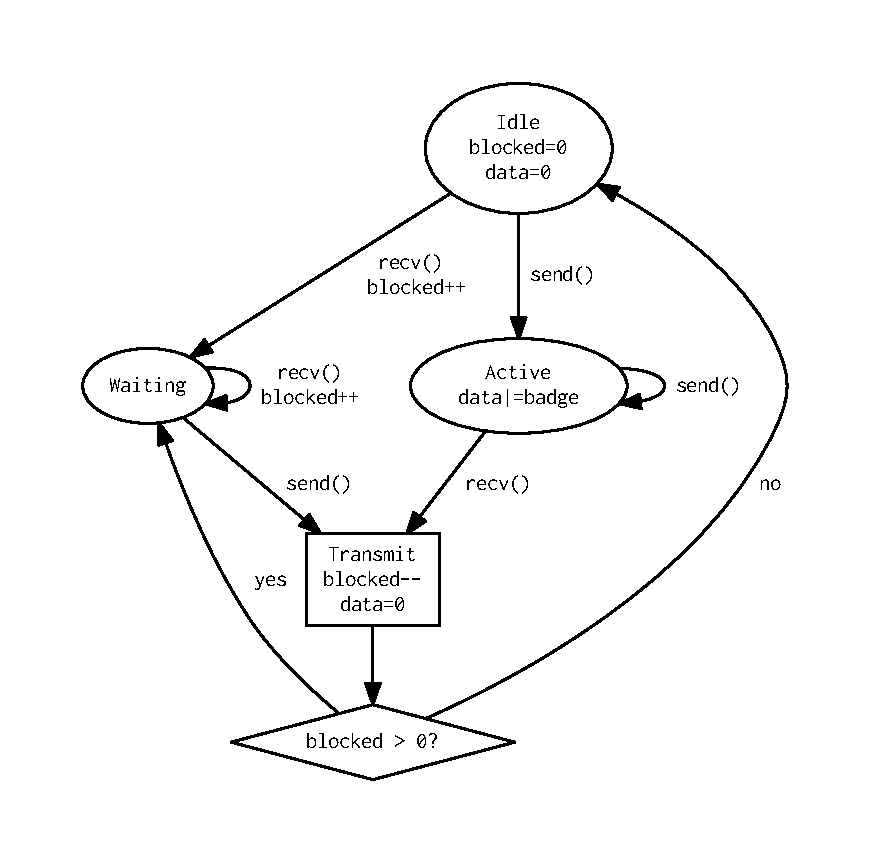
\includegraphics[width=0.8\textwidth]{notification}
    \caption{State diagram Notification object state transitions based on invocations. \code{send} and
    \code{nbsend} correspond to notify in the diagram, want wait corresponds to a \code{recv}.}
    \label{f:notification}
\end{figure}

The data word is set when the first notification arrives, and further invocations continue to bitwise OR the badge and data word
until a thread receives the signal and clears the word. This is illustrated in the notification
state diagram depicted in \cref{f:notification}, and in \cref{f:signal1} which shows the
notification object and TCB interaction.

\Cref{t:notification-system-calls} shows the operations that occur when notification objects are
invoked with relevant system calls. \cref{f:notification} depicts changes in the notification object
state that occur when threads notify and block on notifications. 

\begin{table} 
    \centering
    \rowcolors{2}{gray!25}{}
    \begin{tabularx}{\textwidth}{lX}\toprule
        \emph{System call} & \emph{Action} \\\midrule
        \texttt{send}   & Send a notification, transmitting the badge; do not block. \\ 
        \texttt{nbsend} & As above. \\
        \texttt{recv}   & Wait until a notification is available then receive the data word.  \\
        \texttt{nbrecv} & Poll for a notification, do not block, receive the data word if available. \\
        \bottomrule
    \end{tabularx}
    \caption{System calls and their effects when used on endpoints.}
    \label{t:notification-system-calls}
\end{table}


\subsubsection{Interrupts}

In addition to providing a mechanism for threads to notify each other, notification objects 
also allow threads to synchronise with devices via polling and/or blocking for interrupts. 
IRQHandler capabilities can be associated with a single notification object, via the invocation
\code{set\_notification}, which results in the kernel issuing a notification when an interrupt
occurs. The badge of the notification capability provided to the invocation is bitwise ORed with the
data word when an interrupt is triggered. Further notifications are not issued by the kernel
until the interrupt is acknowledged, using the \code{acknowledge} invocation on IRQHandler
capabilities.

\subsubsection{Notification binding}
\label{s:notification-binding}

Some systems require threads that can receive both notifications and IPC while blocked, in order to
prevent the requirement that services which receive both IPC message and notifications be
multi-threaded.  The mechanism for this is \emph{notification binding} where threads can register a
specific notification capability to receive notifications from while blocked on an endpoint waiting
for IPC. This is done by invoking the TCB with the \code{bind\_notification} invocation, which
establishes a link between a TCB and notification object. Subsequently, if a notification is sent on
that notification object and the TCB receives on any endpoint, that TCB will receive the
notification.  Without notification binding, services require a thread for blocking on a
notification and another thread for blocking on an endpoint, both threads must then synchronise
carefully on any shared data.
Notification binding is illustrated in
\cref{f:signal2}.


\section{Scheduling}

The scheduler in \selfour is used to pick which runnable thread should run next on a specific
processing core, and is a priority-based round-robin scheduler with 256 priorities (0---255). 
At a scheduling decision, the kernel chooses the head of the highest-priority, non-empty list.

Implementation wise, the scheduler consists of an array of lists: one list of ready threads for each
priority level. A two-level bit field is used to track which priority lists contain threads, 
in order to achieve a scheduling decision complexity of $O(1)$. 

The bit field data structure works as follows: the
top-level consists of one word, each bit representing $N$ priorities, where $N$ is 32 or 64
depending on the word size. The second level consists of $256/N$ words, which are indexed by the first bit set in the
top-level bit field. To construct a priority we use the hardware instruction count leading zeros
(\code{CLZ}) to find the highest bit set in the top-level index. We take that index and use
\code{CLZ} on the bottom level bit field corresponding to that index, then construct the priority
from these two values, allowing the highest priority to be found by reading only two words. For
example, on a 32-bit system 
if bit 1 is the highest bit set in the top-level bit field, we index entry 1 in the
bottom level. If bit 5 is the highest bit set in the first entry of the bottom level, we then obtain
$1 * 32 + 5 = 37$ as the highest priority. 
\cref{list:two-lvl-bitmap} shows the logic for the scheduler bit field on 32-bit systems.

\begin{listing}
    \begin{ccode}
uint32_t top_level_index = 0;
uint32_t bottom_level_index[256 / (1u << 5u)];

void addToBitmap(word_t prio) {
    uint32_t l1index = prio >> 5u;
    top_level_bitmap |= (1u << l1index);
    bottom_level_bitmap[l1index] |= (prio & ((1u << 5) - 1u));
}

word_t getHighestPrio(void) {
    uint32_t l1index = 31 - CLZ(top_level_bitmap);
    l2index = 31 - CLZ(bottom_level_bitmap[l1index]));
    return (l1index << 5 | l2index);
}
    \end{ccode}
    \caption{Example algorithms for adding a priority to the scheduler bitmap and extracting the highest
        active priority, on a 32-bit system. Both operations are $O(1)$ and involve two memory
        accesses. 
    \code{CLZ} is the hardware instruction for count leading zeros.}
    \label{list:two-lvl-bitmap}
\end{listing}

\subsection{Scheduler optimisations}

A scheduling decision needs to be made whenever a thread transitions from or to a runnable state.
The majority of thread state transitions occur on IPC, which is critical for performance, 
as can be seen in the simplified thread state diagram shown in \cref{f:thread_state}. 
\begin{figure}[h!tb]
    \centering
    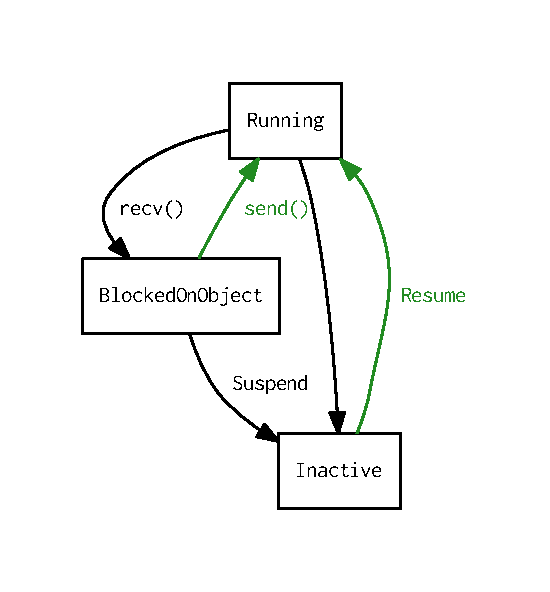
\includegraphics[width=0.6\textwidth]{thread_state}
    \caption{Thread state transitions in \selfour}
    \label{f:thread_state}
\end{figure}
The \code{BlockedOnObject} state in the diagram maps to \code{blockedOn<N>} in the following thread
state definitions:
\begin{itemize}
    \item \code{Running}: This thread is eligible to be picked by the scheduler, and should be in the
        scheduling queues or be the currently running thread.
    \item \code{Inactive} This thread is not runnable, and is not in the scheduler. It has been
        suspended, or possibly never resumed. 
    \item \code{BlockedOnRecv}: This thread is waiting to receive an IPC (or bound notification). 
    \item \code{BlockedOnSend}: This thread is waiting to send an IPC. 
    \item \code{BlockedOnReply}: This thread is blocked on a resume capability, waiting for a reply
        from a \code{call} or fault.
    \item \code{BlockedOnNotification}: This thread is waiting to receive a notification.
\end{itemize}

Several optimisations to the scheduler exist in the kernel for performance, including lazy and benno
scheduling. 
\emph{Lazy} scheduling is used whenever a thread blocks and wakes
another thread at the same time, for example, in the \code{call} system call where the sender is
blocked on the resume capability and the receiver is woken. Lazy scheduling observes that the
current thread must be the highest-priority, runnable thread, and checks if the woken thread is
higher than any other runnable thread by querying the scheduler bit field. If so, the receiver is
directly switched to and the scheduler is avoided all together. Otherwise, the receiver is moved from
the endpoint queue into the scheduling queue and the scheduler called.

\emph{Benno} scheduling, named for its inventor Ben Leslie, removes the current thread from the 
scheduler, changing the invariant that all runnable thread are in the scheduler, to all runnable
threads \emph{except the current thread} are in the scheduler. Consequently, we avoid manipulating the
scheduling queues when doing a direct switch, reducing the cache footprint and resulting in a performance improvement.

The result of these optimisations is that \selfour, like L4 kernels before it, has very fast
\gls{IPC}, compared to non-L4 kernels e.g.\ at least a factor of four in CertiKOS~\citep{Gu_SCWKSC_16}.

\subsubsection{Round-robin}

Kernel time is accounted for in ticks, and each TCB has a timeslice field which represents the number of ticks they are eligible to run. 
This value is decremented every time a timer tick is handled, and when the timeslice is exhausted the thread is appended to the relevant scheduler queue, with a replenished timeslice.
Threads can surrender their current tick using the \code{yield} system call, which places the thread
at the end of the scheduler queue.

When threads communicate with a service over \gls{IPC}, the TCB of the thread providing the service
is charged for any ticks that occur while that service is active. As a result isolation in shared
server is not possible: clients are not charged for their execution time. 

\subsubsection{Priorities}

Like any priority-based kernel without temporal isolation mechanisms, time is only guaranteed to the highest priority threads.
Priorities in \selfour act as informal capabilities: threads cannot create threads at priorities higher than their current priority, but can create threads at the same or lower priorities.
If threads at higher priority levels never block, lower priority threads in the system will not run.
As a result, a single thread running at the highest priority has access to 100\% of processing time.

\subsection{Domain scheduler}

In order to provide confidentiality~\citep{Murray_MBGBSLGK_13} \selfour provides a top-level hierarchical scheduler
which provides static, cyclical scheduling of scheduling partitions known as \emph{domains}. 
Domains are statically configured at compile time with a cyclic schedule, and are non-preemptible
resulting in completely deterministic scheduling of domains.
Each domain has its own priority scheduler, with lists per priority and a bit field structure, which is switched deterministically when a domain's
ticks expire. 
Threads are assigned to domains, and threads are only scheduled when their domain is active.
Cross-domain \gls{IPC} is delayed until a domain switch, and \texttt{yield} between domains is not
possible. When there are no threads to run while a domain is scheduled, a domain-specific idle thread will run until a switch occurs.

The domain scheduler is consistent with that specified by the \citet{ARINC653} standard, and 
can be leveraged to achieve temporal isolation. However, since domains cannot be
preempted, it is only useful for cyclic, non-preemptive scheduling with scheduling order and
parameters computed-offline.
In such a scenario each real-time task could be mapped to its own domain, and each task would run for its specified time before the domain scheduler switched to the next thread.
Any unused time in a domain would be wasted, and spent in the idle thread.

Such a scheduler is only suitable for closed systems and results in low system utilisation.
Dynamic real-time applications with shared resources and high system utilisation are not compatible
with the domain scheduler, as they require preemption.

\subsection{Real-time support}

We introduced basic \selfour concepts and terminology, and investigated mechanisms that effect
timing behaviour in the kernel: the scheduler, domains, priorities, \code{yield} and IPC. 
In this section we will look at how real-time scheduling could be implemented with those mechanisms.

There are several options for implementing a real-time scheduler in the current version of \selfour:
leveraging the domain scheduler, using the priority scheduler or implementing a scheduling component
to run at user-level. We explore these by explaining how a fixed-priority scheduler can be
implemented with each technique, and explore the limitations. 

%explain how to use the domain scheduler for RM
A basic cyclic executive, as introduced in \cref{s:cyclic-executive} can be implemented using the
domain scheduler by mapping domains directly to task frames. This approach only works for closed
systems with offline scheduling. An optimal scheduler like \gls{FPRM} is not possible to implement
with domains as they are not preemptible. 

% FPRM with priority scheduler
The priority scheduler can be leveraged to implement \gls{FPRM}, by mapping \selfour priorities to 
rate-monotonic priorities. 
However, this requires complete trust in every thread in the system, as there is no mechanism for
temporal isolation: if one thread executes for too long, other threads will miss their deadlines.
Essentially the only thread with a guaranteed CPU allocation is the highest priority thread, which
under rate-monotonic priority assignment is not the most critical thread in the system, but the
thread with the highest rate.  Additionally, periodic threads driven by timer interrupts rather than
events would need to share a user-level timer.

% trusted component at user-level
To build a dynamic system with temporal isolation and high CPU utilisation, one could provide a 
high-priority scheduling component which implements \gls{FPRM} at user-level. This task would manage a
time-service for timeouts and monitor task execution, preempting tasks before they exceed their
declared \gls{WCET}. On task completion, tasks would RPC the scheduler in order to dispatch
a new task.
However, since the timer component would need to maintain accounting information and track the currently running thread, it would need to be invoked for every single scheduling operation.
This is prohibitively expensive, as it results in doubled context switching time and increased number of system calls for thread management.

\begin{table}
	\centering
    \rowcolors{3}{}{gray!25}
    \begin{tabularx}{\textwidth}{Xllll} \toprule
        & \emph{Temporal}   & \emph{Utilisation} & \emph{Low kernel} & \emph{Dynamic}\\
        & \emph{isolation}  &                    & \emph{overheads} & \\  
        \midrule
Domain scheduler          & \yes               & \no         & \yes        & \no    \\
Priority scheduler        & \no                & \yes        & \yes        & \yes   \\
Scheduling component   & \yes               & \yes        & \no         & \yes   \\
        \bottomrule
	\end{tabularx}
	 \caption{Comparison of existing \selfour scheduling options.}
	 \label{tab:nothing-ticks-all-boxes}
\end{table}

\Cref{tab:nothing-ticks-all-boxes} shows a comparison of all the available scheduling options in
the current version of \selfour---no option provides all the qualities we require.

\section{Summary}

In this chapter we have provided an overview of \selfour concepts, including capabilities, system
calls, resource management, communication and scheduling. We conclude that current real-time
scheduling support is deficient, and temporal isolation is not possible over shared server IPC.  

In the next section we will outline our model for a more principled approach to managing time by
extending the baseline \selfour model presented in this chapter. We appeal to resource kernel
principles where time is treated as a first-class resource, with the aim of support diverse task
sets, including those for mixed-criticality systems.
